\documentclass[aspectratio=169]{beamer}
\usepackage{animate}
\usepackage{graphicx}
\usepackage{amsmath} % Added for math environments
\usepackage{url}     % Added for \url command
%\usepackage{apacite} % Added for APA citation style
\usepackage[style=apa, backend=biber]{biblatex}
\usepackage{microtype} % Added to improve justification

% Optional: Add a theme
\usetheme{Madrid}

% Add bibliography resource (make sure the path is correct)
\addbibresource{../references.bib}

\title[Tech Demo]{Technical Demo: \\ Graph Representation Learning for Geography} % Added "for Geography"
\author{Yuta Sato}
\institute{University of Liverpool} % Optional: Add affiliation
\date{May 7th, 2025}

\begin{document}

\frame{\titlepage}

\begin{frame}
    \frametitle{Agenda}
    \begin{itemize}
        \item What is graph?
        \item Examples of Graphs in Geography
        \item What is Graph Representation Learning
        \item Why GNNs?
        \item Message Passing Framework
        \item Notable GNN Models
        \item GNNs in Geographic Data Science
        \item Technical Demonstration
    \end{itemize}
    \textbf{Note:} This presentation provides an overview and does not delve deeply into Graph Theory, Network Science, or specific Deep Learning implementation details.
\end{frame}

\section{Introduction}
\begin{frame}
    \frametitle{What is a Graph? (1/2)}
    \begin{itemize}
        \item A graph is a mathematical structure consisting of:
        \begin{itemize}
            \item \textbf{Nodes (vertices)}: represent entities
            \item \textbf{Edges}: represent relationships between entities
        \end{itemize}
        \item Real-world examples:
        \begin{itemize}
            \item \textbf{Social networks}: Users (nodes) and friendships (edges)
            \item \textbf{Molecules}: Atoms (nodes) and bonds (edges)
            \item \textbf{Internet}: Global IP address (nodes) and web links (edges)
        \end{itemize}
        \begin{center}
            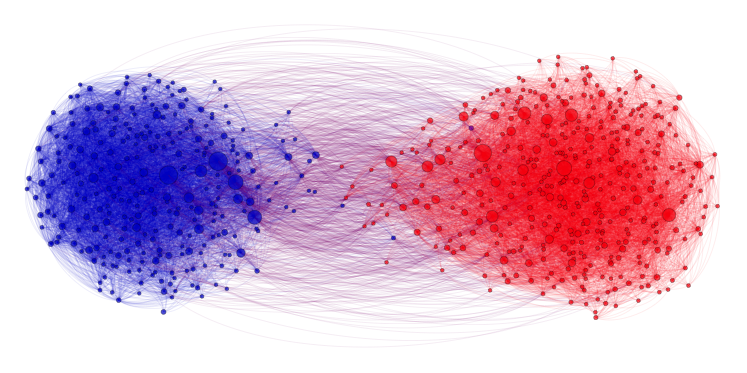
\includegraphics[width=0.45\textwidth,height=0.5\textheight,keepaspectratio]{../images/social_network.png}
            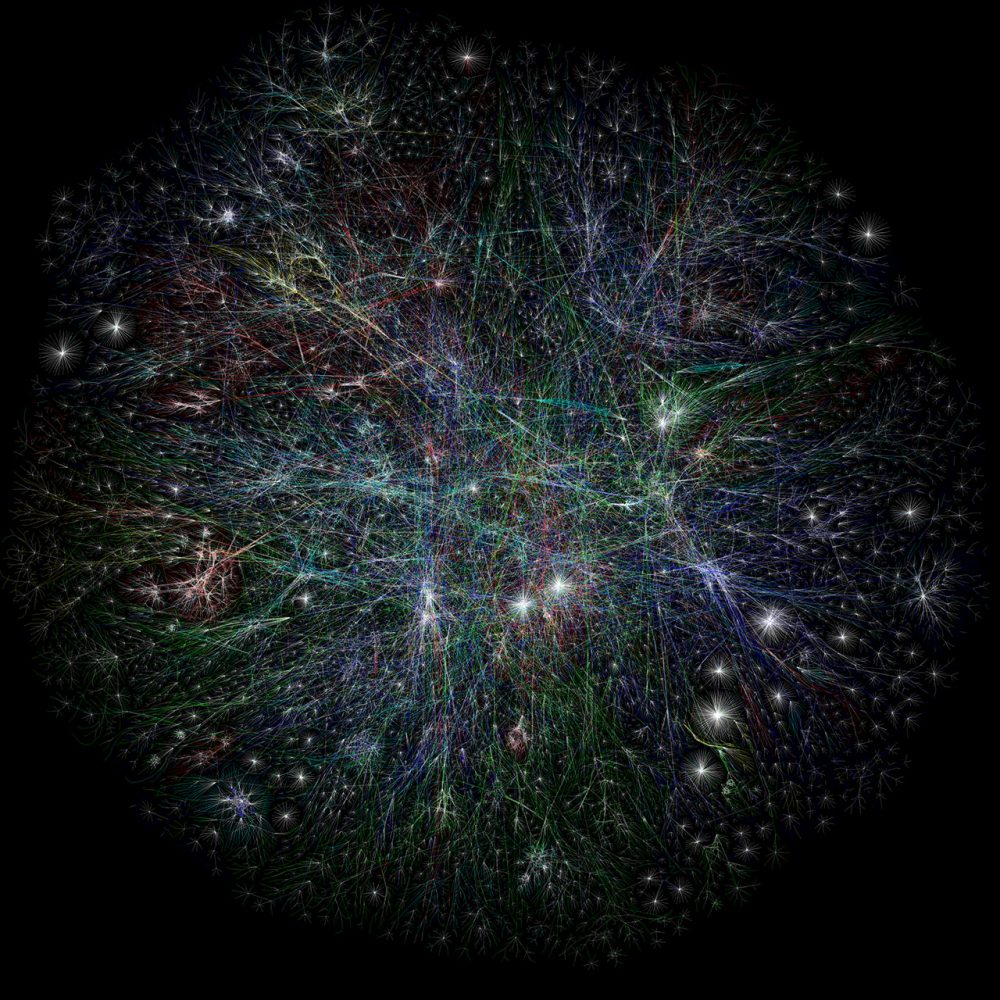
\includegraphics[width=0.45\textwidth,height=0.5\textheight,keepaspectratio]{../images/internet.jpg}
        \end{center}            
    \end{itemize}
\end{frame}

\begin{frame}
    \frametitle{What is a Graph? (2/2)}
    \begin{itemize}
        \item \textbf{Heterogeneous Graphs}:
        \begin{itemize}
            \item Multiple types of nodes and/or edges
            \item Different node/edge types may have different feature structures
        \end{itemize}
    \end{itemize}
    \begin{center}
        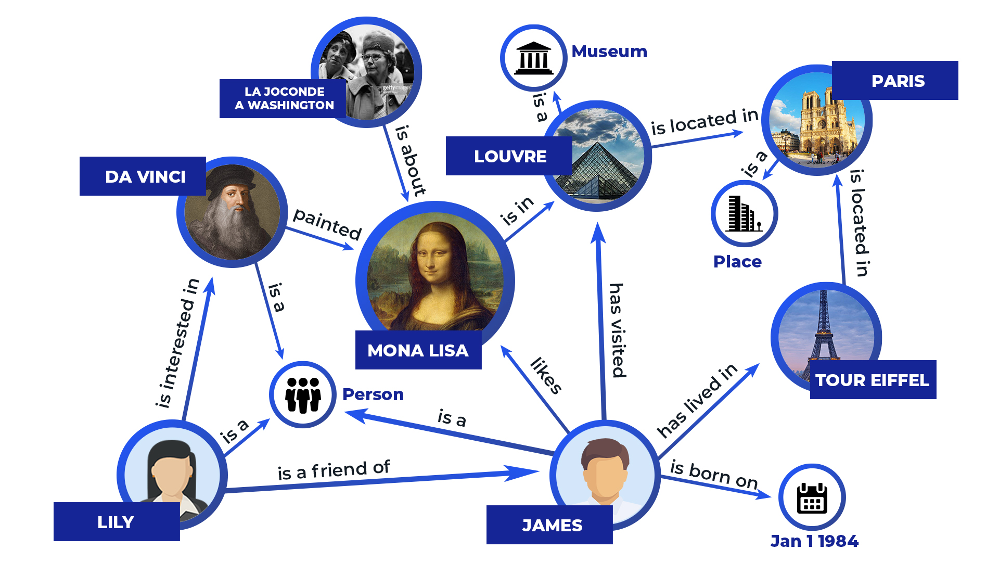
\includegraphics[width=0.7\textwidth]{../images/hetero_graph.png}
    \end{center}     
\end{frame}

\begin{frame}
    \frametitle{Examples of Graphs in Geography (1/3): Streets}
    \begin{itemize}
        \item \textbf{Street Networks}:
        \begin{itemize}
            \item In general planar and can be represented as primary and dual graphs \parencite{porta_network_2006}
            \item Primal Graph (nodes: intersections/segments, edges: streets)
            \item Dual Graph (nodes: road segments, edges: intersections)
        \end{itemize}
    \end{itemize}
    \begin{center}
        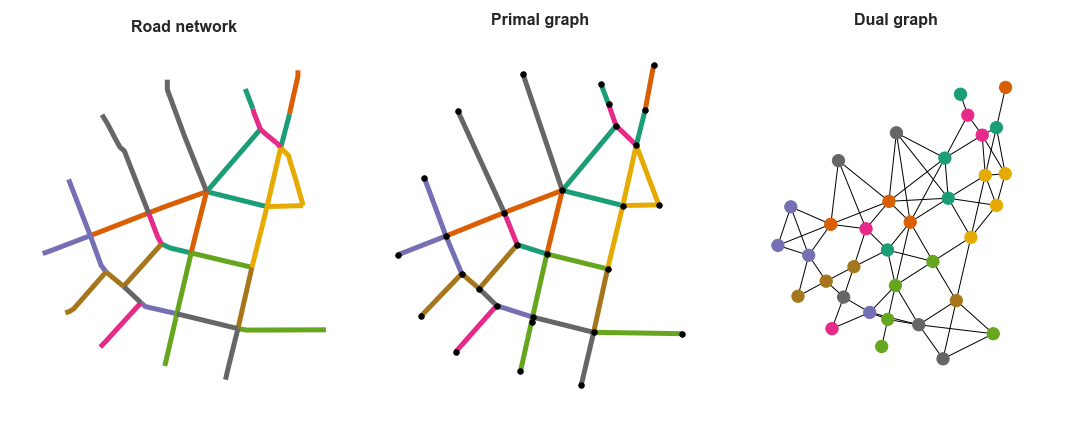
\includegraphics[width=0.8\textwidth]{../images/primal_dual.png}
    \end{center}
\end{frame}

\begin{frame}
    \frametitle{Examples of Graphs in Geography (2/3): Mobility}
        \begin{itemize}
            \item \textbf{Origin-Destination (OD) Matrices}:
            \begin{itemize}
            \item Nodes: locations/zones, edges: movement flows
            \item Weights: trip frequency/volume, mode share
            \end{itemize}
            \item \textbf{Transportation Networks}:
            \begin{itemize}
            \item Nodes: locations/zones, edges: transportation routes
            \item Weights: distance, travel time, cost
            \end{itemize}  
        \end{itemize}
        \begin{center}
            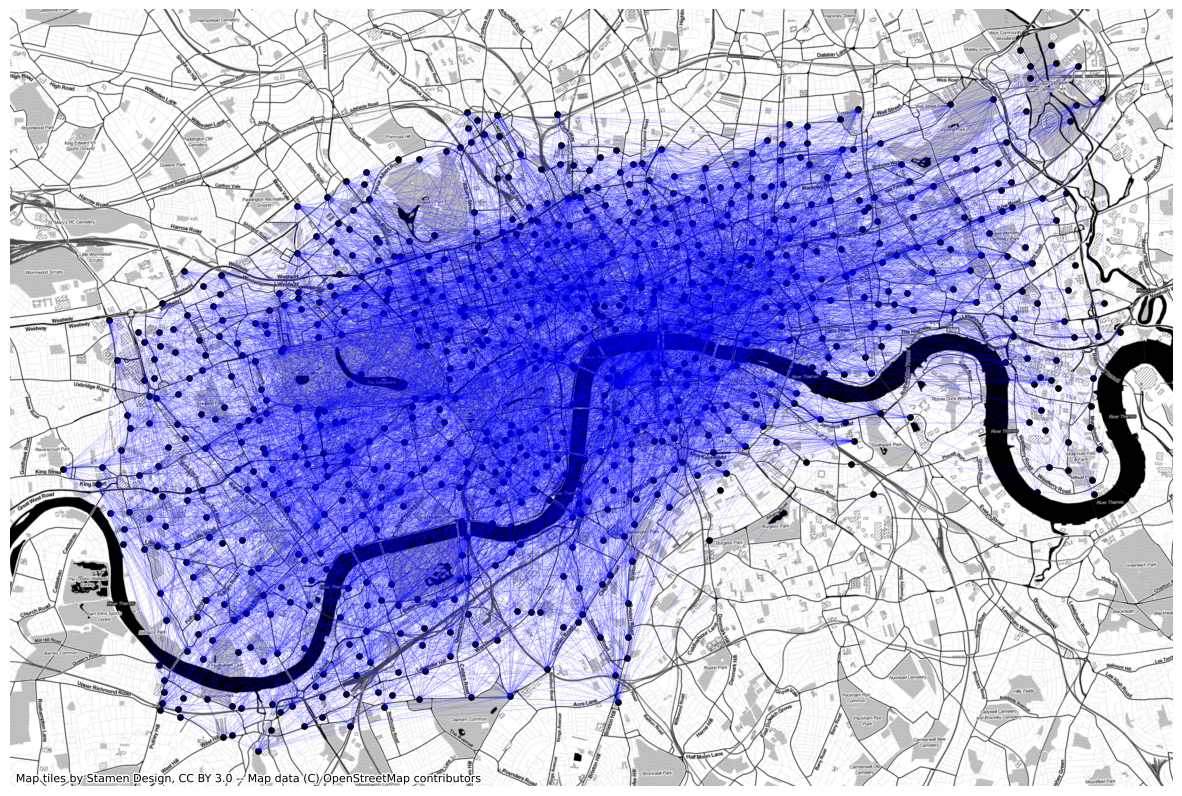
\includegraphics[width=0.45\textwidth,height=0.5\textheight,keepaspectratio]{../images/bike_share.png}
            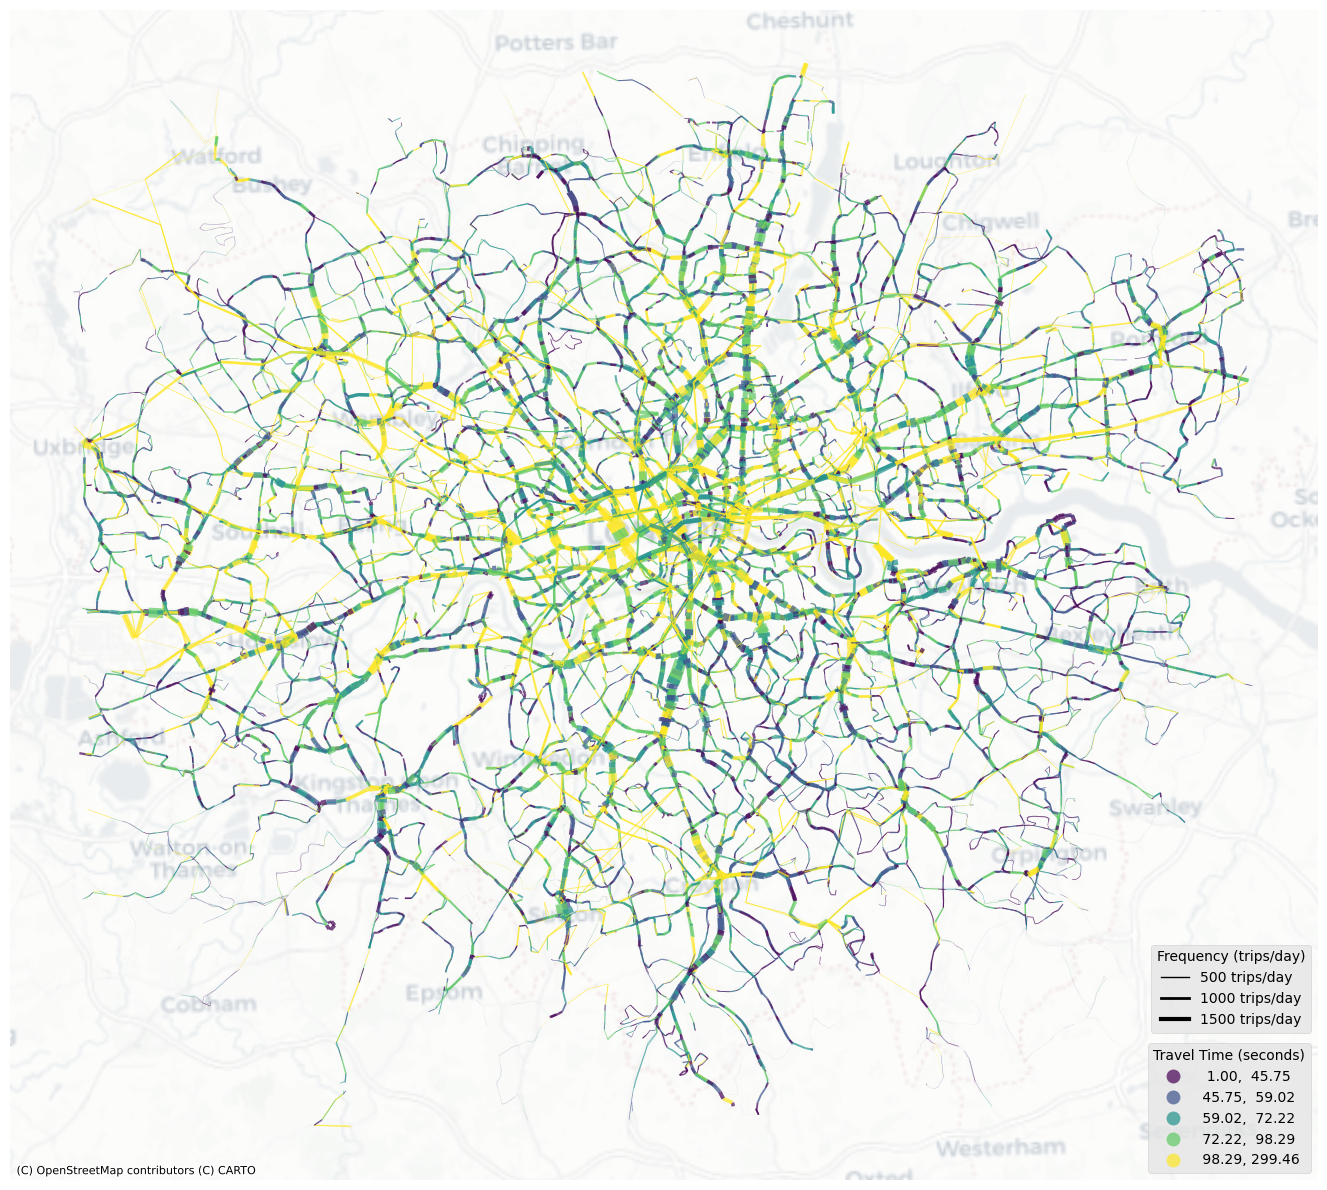
\includegraphics[width=0.45\textwidth,height=0.5\textheight,keepaspectratio]{../images/trav_sum_network_overview.png}
        \end{center}
\end{frame}

\begin{frame}
    \frametitle{Examples of Graphs in Geography (3/3): Spatial Contiguity / Proximity}
    \begin{itemize}
        \item Spatial Contiguity/Proximity Networks:
        \begin{itemize}
            \item Regions/areas (nodes) connected by shared boundaries or proximity (edges)
        \end{itemize}
    \end{itemize}
    \begin{center}
        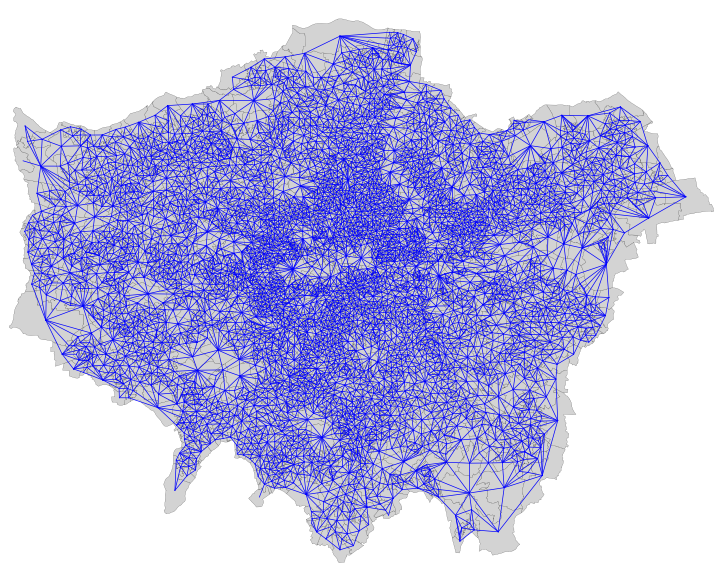
\includegraphics[width=0.5\textwidth]{../images/contiguity.png}
    \end{center}    
\end{frame}

\begin{frame}
    \frametitle{What is Graph Representation Learning? (1/2)}
    \begin{itemize}
        \item \textbf{Graph Representation Learning}:
        \begin{itemize}
            \item Machine learning models that maps nodes/graphs to vectors in $d$-dimensional embedding space (Euclidean)
            \item Node prediction ($f_n: \{\mathcal{G}_i\} \to \mathbb{R}^{n \times d}$)
            \item Edge prediction ($f_e: \{\mathcal{G}_i\} \to \mathbb{R}^{n \times n \times d}$)
            \item Graph prediction ($f_g: \{\mathcal{G}_i\} \to \mathbb{R}^{d}$)
        \end{itemize}
        \begin{center}
            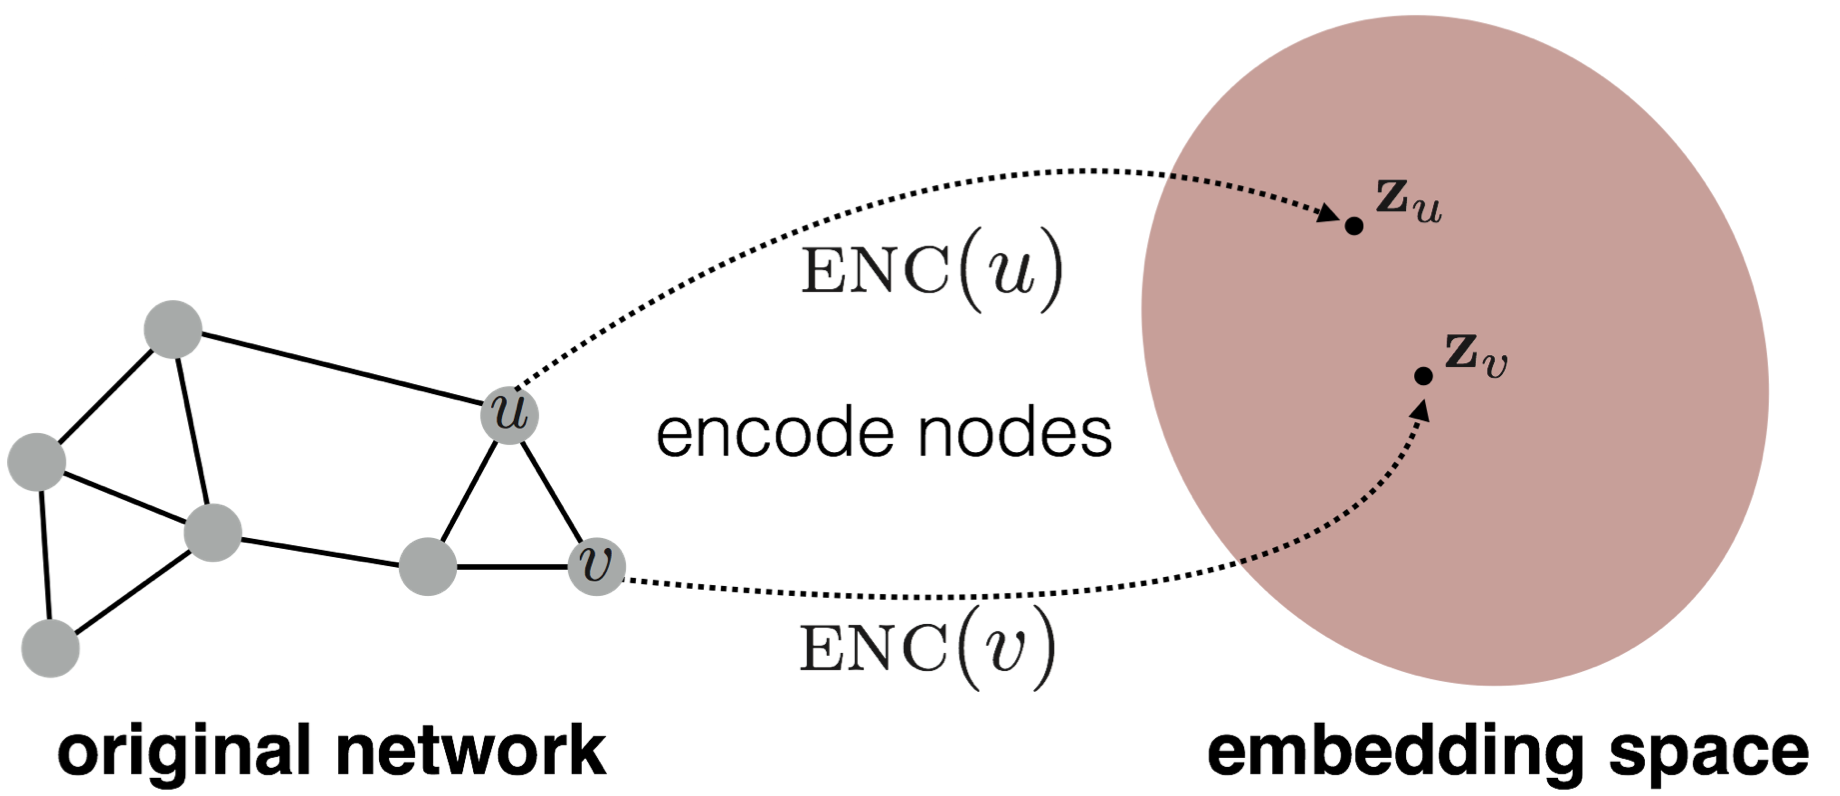
\includegraphics[width=0.5\textwidth]{../images/node_embeddings} % Image path needs verification
        \end{center}
    \end{itemize}
\end{frame}


\begin{frame}
    \frametitle{What is Graph Representation Learning? (2/2)}
    \begin{itemize}
        \item \textbf{Graph Neural Networks (GNNs)}:
        \begin{itemize}
            \item Deep learning models for graph-structured data
            \item Learn representations through \textbf{message passing framework}
            \item Update node features by aggregating neighbor information
        \end{itemize}
        \begin{center}
            \animategraphics[autoplay,loop,width=0.3\textwidth]{12}{../images/message_passing_framework-}{0}{54}
        \end{center}
    \end{itemize}
\end{frame}


\begin{frame}
    \frametitle{Why GNNs?} % Title updated to match Agenda
    \begin{itemize}
        \item Traditional ML struggles with graph data:
        \begin{itemize}
            \item Fixed-size input assumption (e.g., images, sequences)
            \item Order-dependent (graphs are inherently unordered)
            \item Fails to capture relational structure explicitly
        \end{itemize}
        \item GNNs offer key advantages:
        \begin{itemize}
            \item Handle irregular, non-Euclidean graph structures
            \item Permutation invariant/equivariant (node order doesn't matter)
            \item Leverage node features, edge features, and topology simultaneously
        \end{itemize}
    \end{itemize}
        \begin{center}
            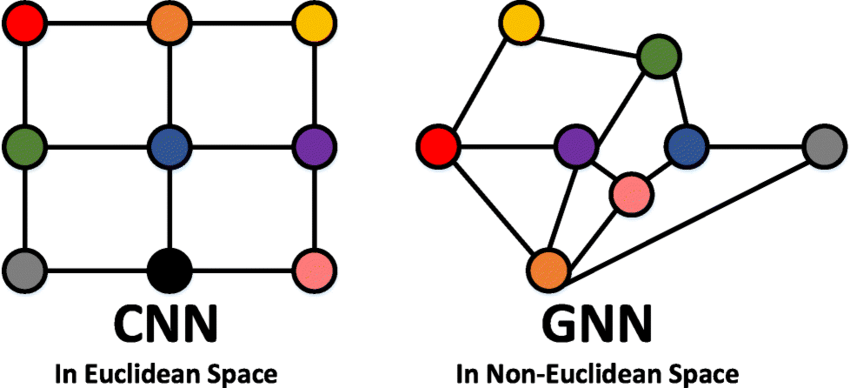
\includegraphics[width=0.5\textwidth]{../images/cnn_vs_gnn.png} % citation removed
        \end{center}
    \end{frame}

\begin{frame}
    \frametitle{Message Passing Framework}
    \begin{center}
        \begin{itemize}
            \item \textbf{Core idea}: Nodes iteratively aggregate information from neighbors to update their own representations.
            \item \textbf{General Formulation} (Layer $k$ to $k+1$):
             % Resized equation slightly smaller
                \begin{center}                
                \resizebox{0.5\textwidth}{!}{
                $\displaystyle
                    \mathbf{h}_v^{(k+1)} = \gamma^{(k)} \left( \mathbf{h}_v^{(k)}, \underset{u \in \mathcal{N}(v)}{\square^{(k)}} \phi^{(k)} \left( \mathbf{h}_v^{(k)}, \mathbf{h}_u^{(k)} \right) \right)
                $
                }
            \end{center}
            \begin{itemize}
                \item $\mathbf{h}_v^{(k)}$: Representation (hidden state) of node $v$ at layer $k$.
                \item $\mathcal{N}(v)$: Set of neighbors of node $v$.
                \item $\phi^{(k)}$: Message function (computes message from neighbor $u$ to $v$). Often involves learnable weights $\mathbf{W}^{(k)}$.
                \item $\square^{(k)}$: Aggregation function (combines messages from neighbors, e.g., sum, mean, max). Must be permutation invariant.
                \item $\gamma^{(k)}$: Update function (combines aggregated message with node's previous state, often involves activation). E.g., MLP + Activation($\sigma(x) = \frac{1}{1+e^{-x}}$, ReLU=$\max(0,x)$).
            \end{itemize}
        \end{itemize}
    \end{center}
\end{frame}

\section{Notable GNN Models (1/3)} % Section title updated
\begin{frame}
    \frametitle{Notable GNN Models (1/3)}
    \begin{itemize}
        \item \textbf{Graph Convolutional Networks (GCNs)} \parencite{kipf2016semi}: 
        \begin{itemize}
            \item Aggregates neighbor features equally (often mean aggregation).
        \end{itemize}
        \item \textbf{Graph Attention Networks (GATs)} \parencite{velivckovic2017graph}:
        \begin{itemize}
            \item Assigns different importance (attention weights) to neighbors during aggregation.
        \end{itemize}
        \begin{center}
            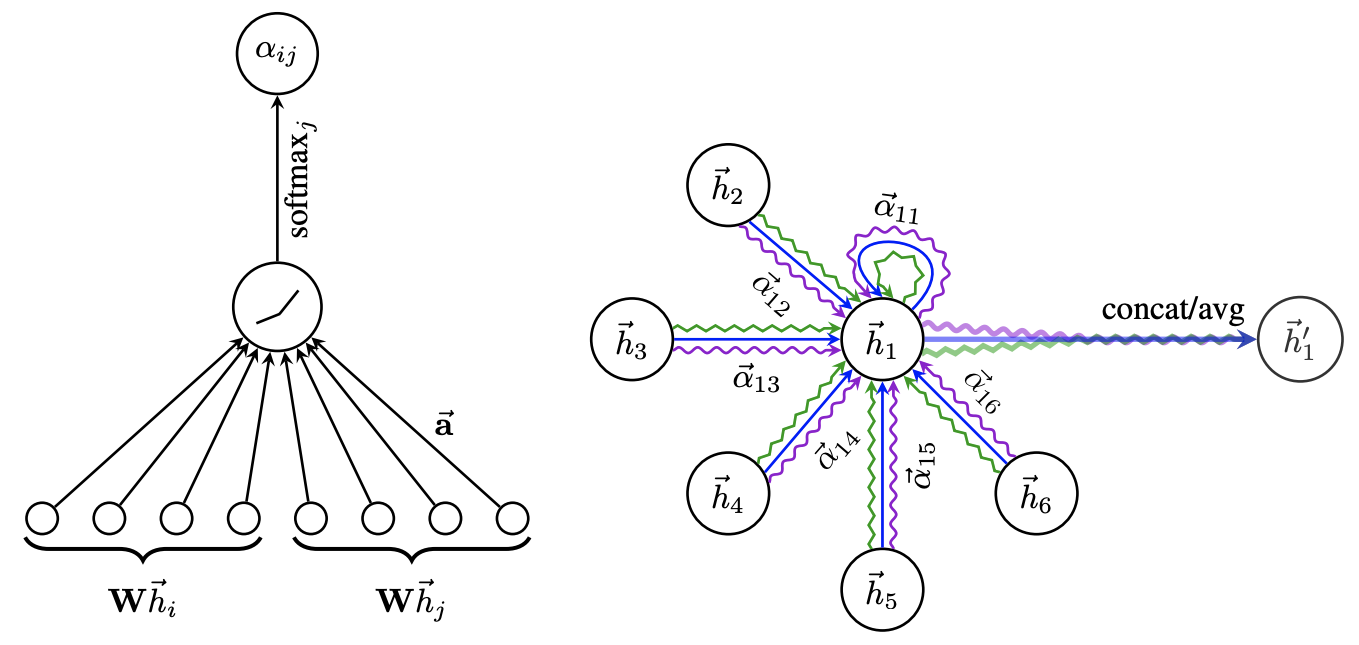
\includegraphics[width=0.4\textwidth]{../images/graph_attention_networks.png}
        \end{center}
    \end{itemize}
\end{frame}

\section{Notable GNN Models (2/3)}
\begin{frame}
    \frametitle{Notable GNN Models (2/3)}
    \begin{itemize}
        \item \textbf{GraphSAGE} \parencite{hamiltonyl17}:
        \begin{itemize}
            \item Scalable GNN that samples a fixed-size neighborhood for each node.
        \end{itemize}
        \begin{center}
            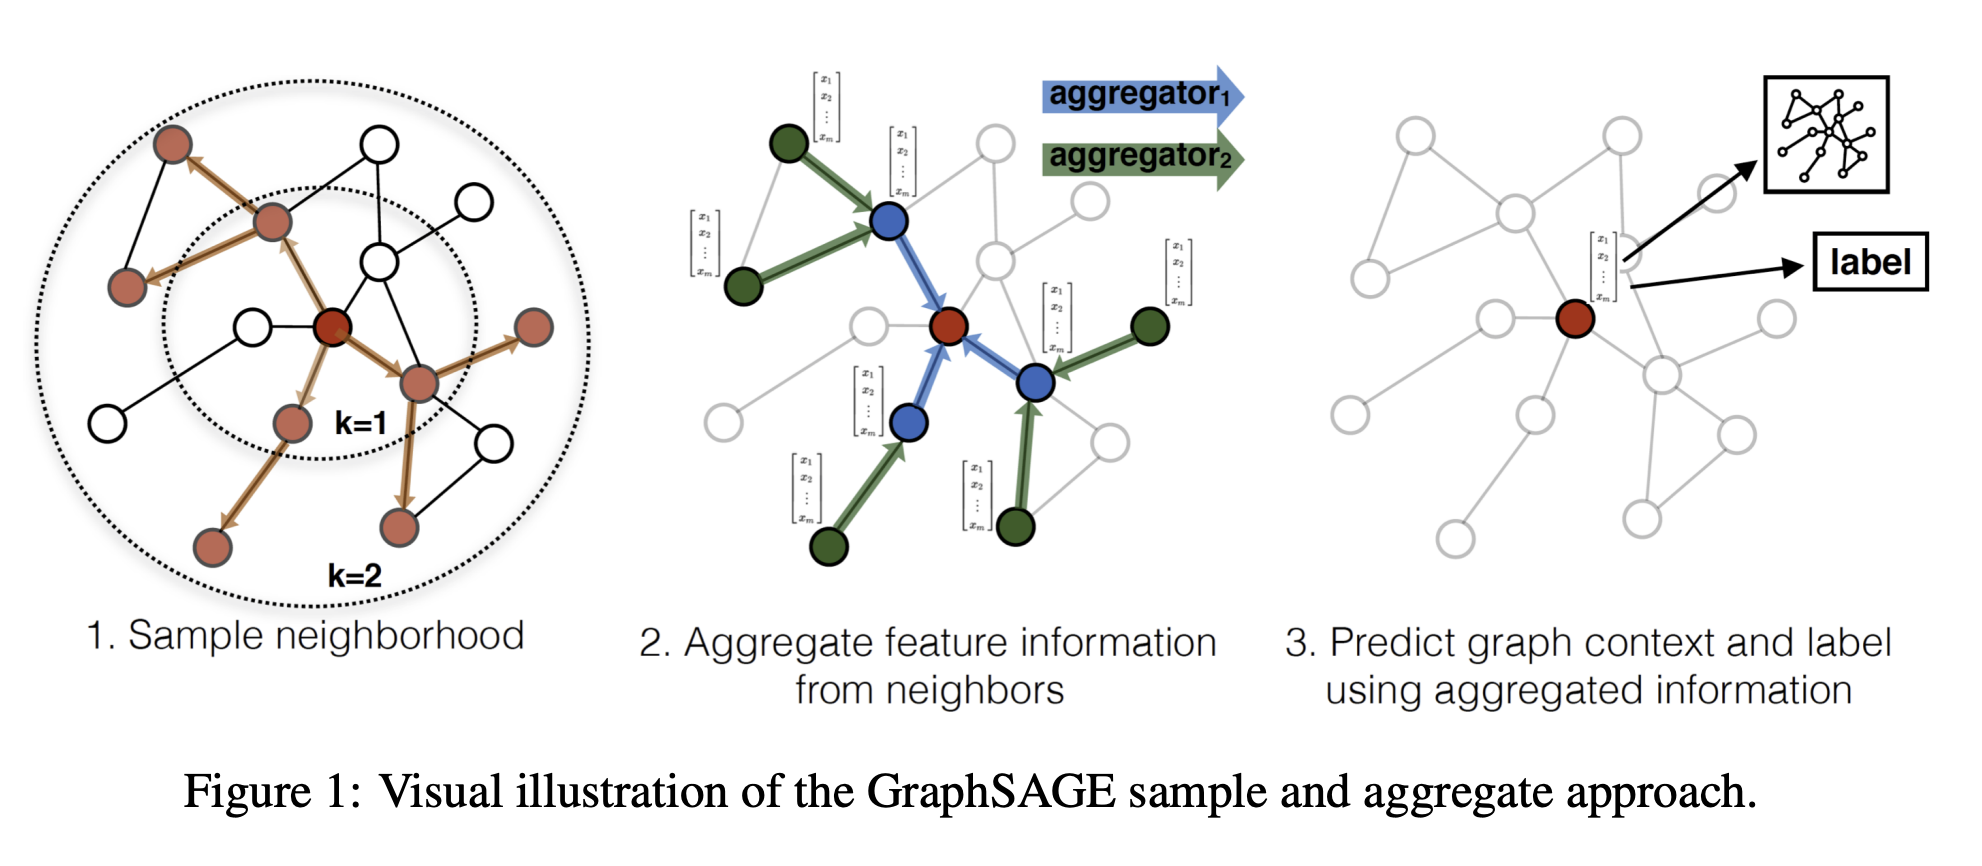
\includegraphics[width=0.4\textwidth]{../images/graphsage.png}
        \end{center}
        
        \item \textbf{Graph Transformers} \parencite{yun2019graph}:
        \begin{itemize}
            \item Uses self-attention over all nodes (or sampled nodes) to capture global dependencies, inspired by NLP Transformers.
        \end{itemize}
    \end{itemize}
\end{frame}

\section{Notable GNN Models (3/3)}
\begin{frame}
    \frametitle{Notable GNN Models (3/3)}
    \begin{itemize}
        \item \textbf{Graph Autoencoder (GAE)} \parencite{kipf2016variationalgraphautoencoders}: % citation removed
        \begin{itemize}
            \item Unsupervised: Learn compressed node embeddings by encoding the graph structure (and features) and decoding to reconstruct it (often the adjacency matrix).
        \end{itemize}
        \begin{center}
            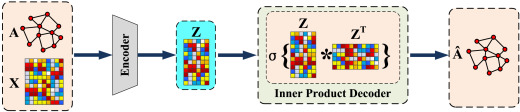
\includegraphics[width=0.6\textwidth]{../images/GAE.png} % Consider citing the source if image isn't original
        \end{center}
        \item \textbf{Graph Pooling} \parencite{liu2023graphpoolinggraphneural}: % citation removed
        \begin{itemize}
            \item Down-samples the graph (reduces nodes) to create coarser representations, analogous to pooling in CNNs. Hierarchical or global.
        \end{itemize}
        \begin{center}
            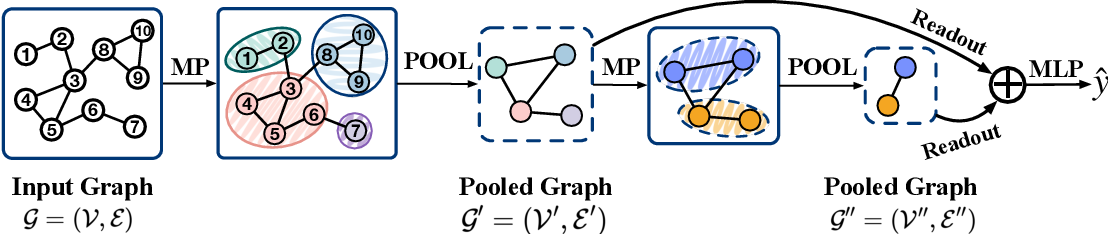
\includegraphics[width=0.6\textwidth]{../images/graph_pooling.png} % Consider citing the source if image isn't original
        \end{center}
    \end{itemize}
\end{frame}

\begin{frame}
    \frametitle{GNNs in Geographic Data Science (1/3)}
    \begin{itemize}
        \item \textbf{Example: Urban Structure Embedding} \parencite{fan2024neural}
        \begin{itemize}
            \item \textbf{Data:} OD matrix (mobility flows) for 16 US cities (nodes: 4km $\times$ 4km grid cells, edges: OD).
            \item \textbf{Features:} Node: Census demographics, POIs. Edge: Trip counts.
            \item \textbf{Task:} Link prediction (mobility flow) using GCN. Node embeddings were clustered by Hierarchical Clustering to reveal functional urban zones.
            \item \textbf{Finding:} GNN embeddings captured spatial structures related to urban functions (residential, commercial etc.).
        \end{itemize}
        \begin{center}
            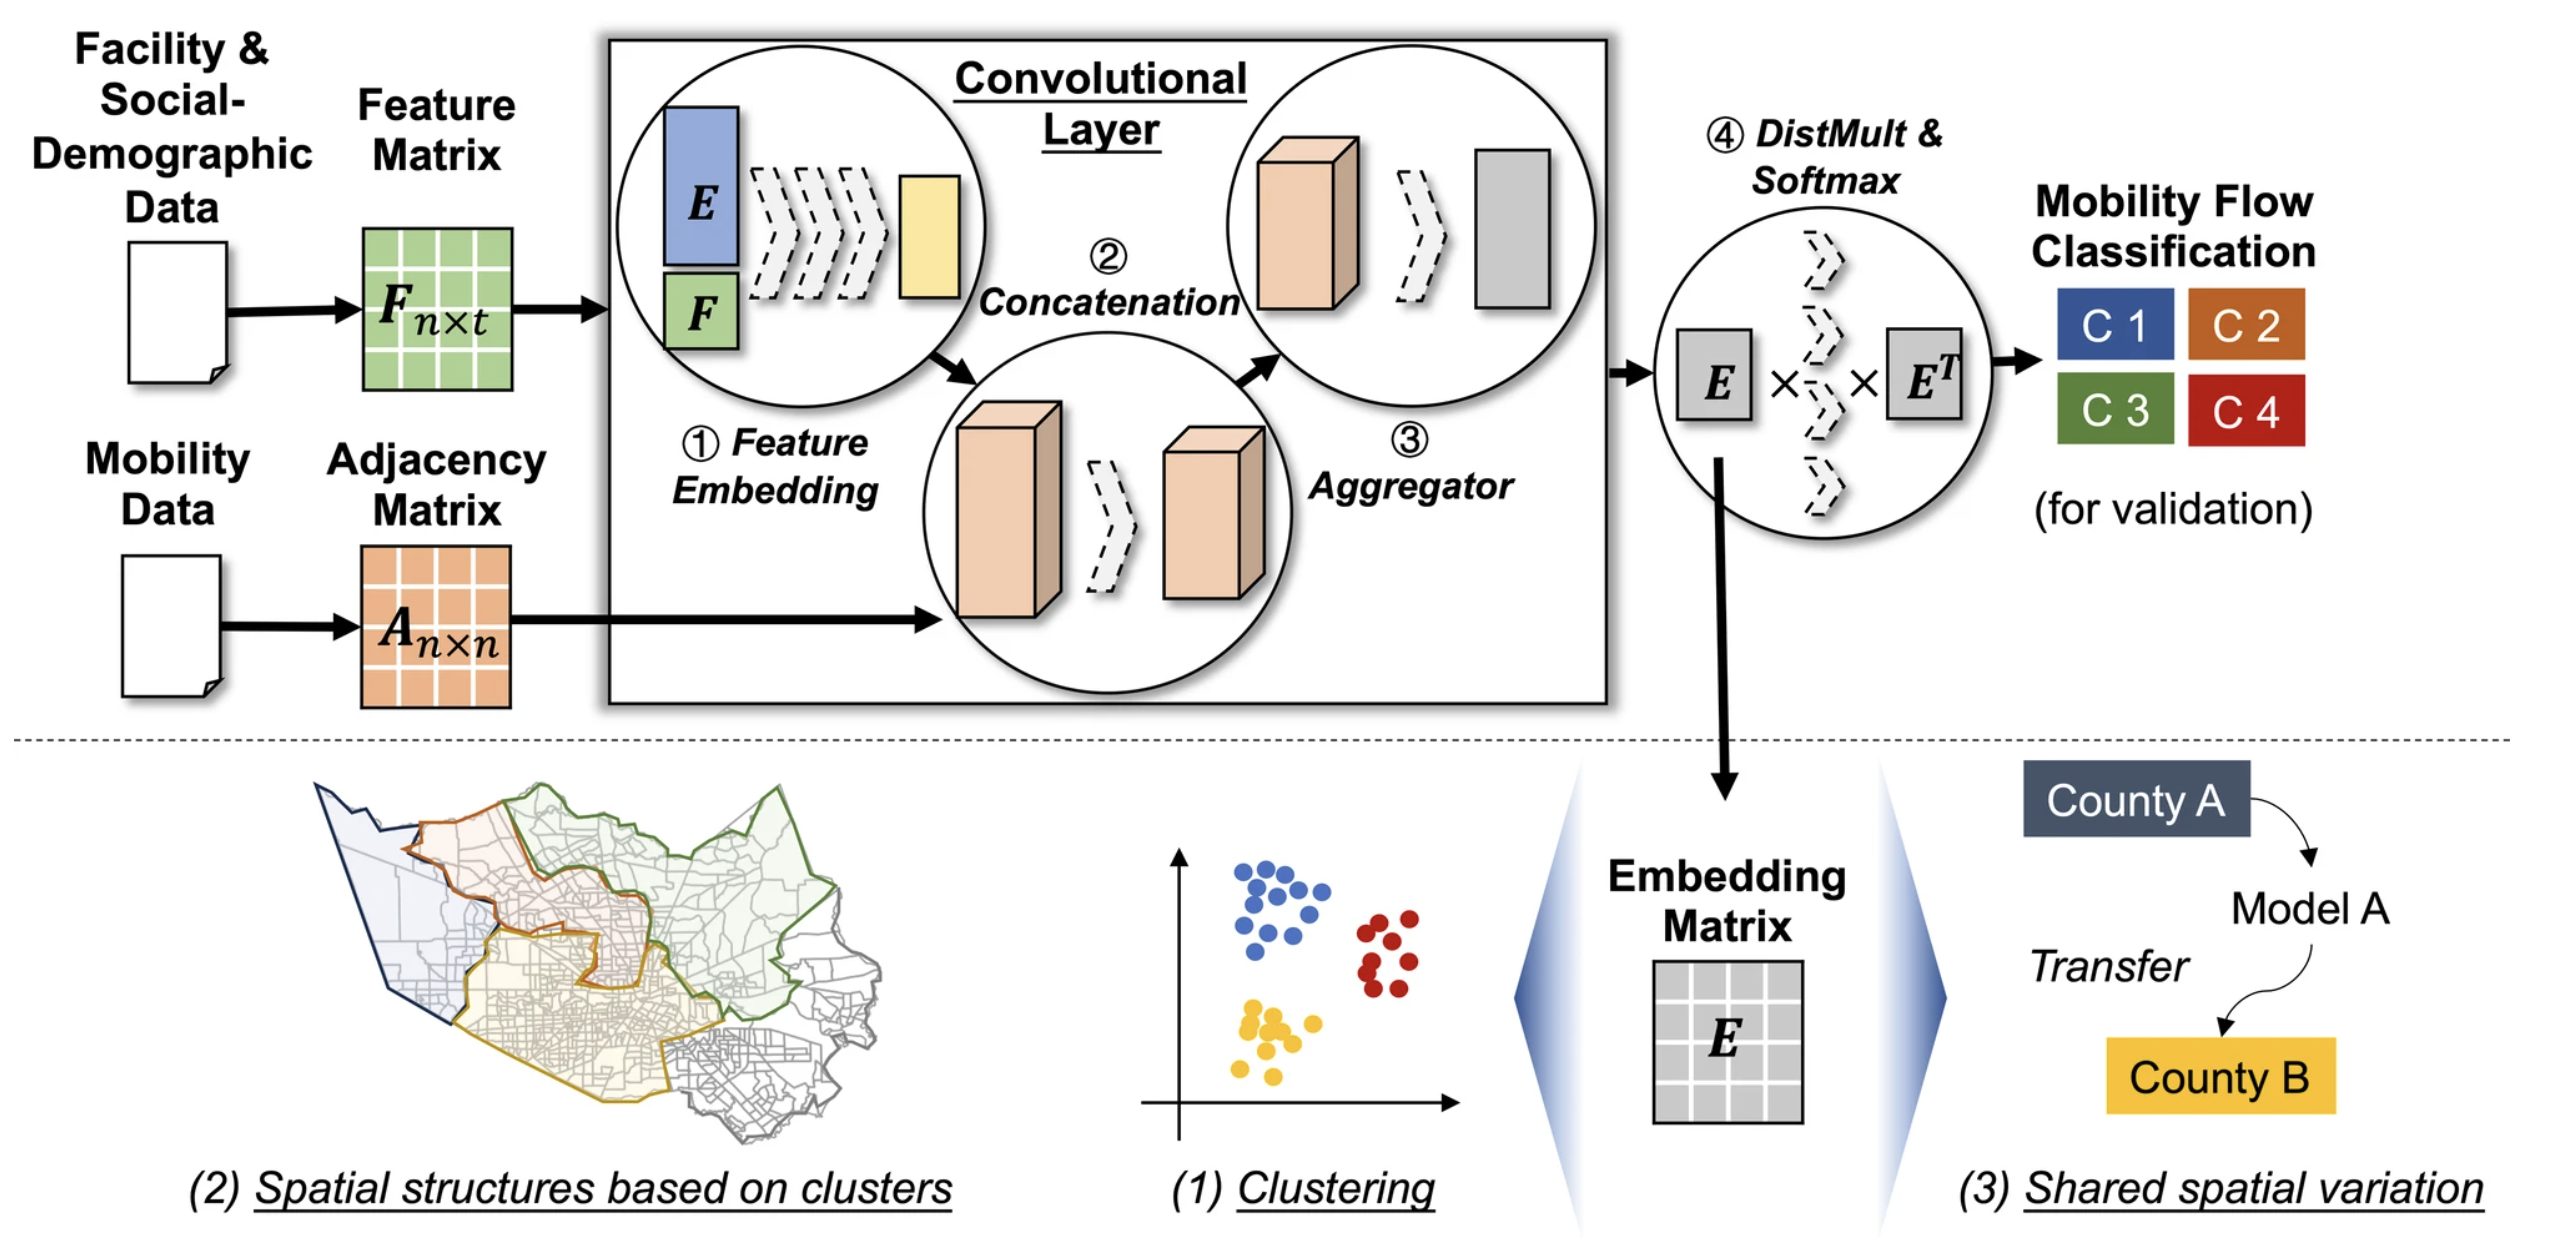
\includegraphics[width=0.5\textwidth]{../images/Fan_and_Mostafavi_2024.png} % citation removed
        \end{center}
    \end{itemize}
\end{frame}

\begin{frame}
    \frametitle{GNNs in Geographic Data Science (2/3)} % Add content here!
    \begin{itemize}
        \item \textbf{Example: Geodemographic Clustering} \parencite{De_Sabbata02122023} 
        \begin{itemize}            
            \item \textbf{Data:} Greater London's administrative boundary in 2011 UK Census (nodes: Output Areas, edges: Queen-contiguity / KNN / distance threshold)
            \item \textbf{Features:} Node: Census variables (167 z-scores, 60 k-vars). Edge: None
            \item \textbf{Task:} Geodemographic clustering by GAE with GCN / GAT layers (Node embeddings clustered by k-means and spatial fuzzy c-means)
            \item \textbf{Finding:} GAE performed similarly to classic approaches on class homogeneity metrics while providing higher spatial clustering
        \end{itemize}
        \begin{center}
            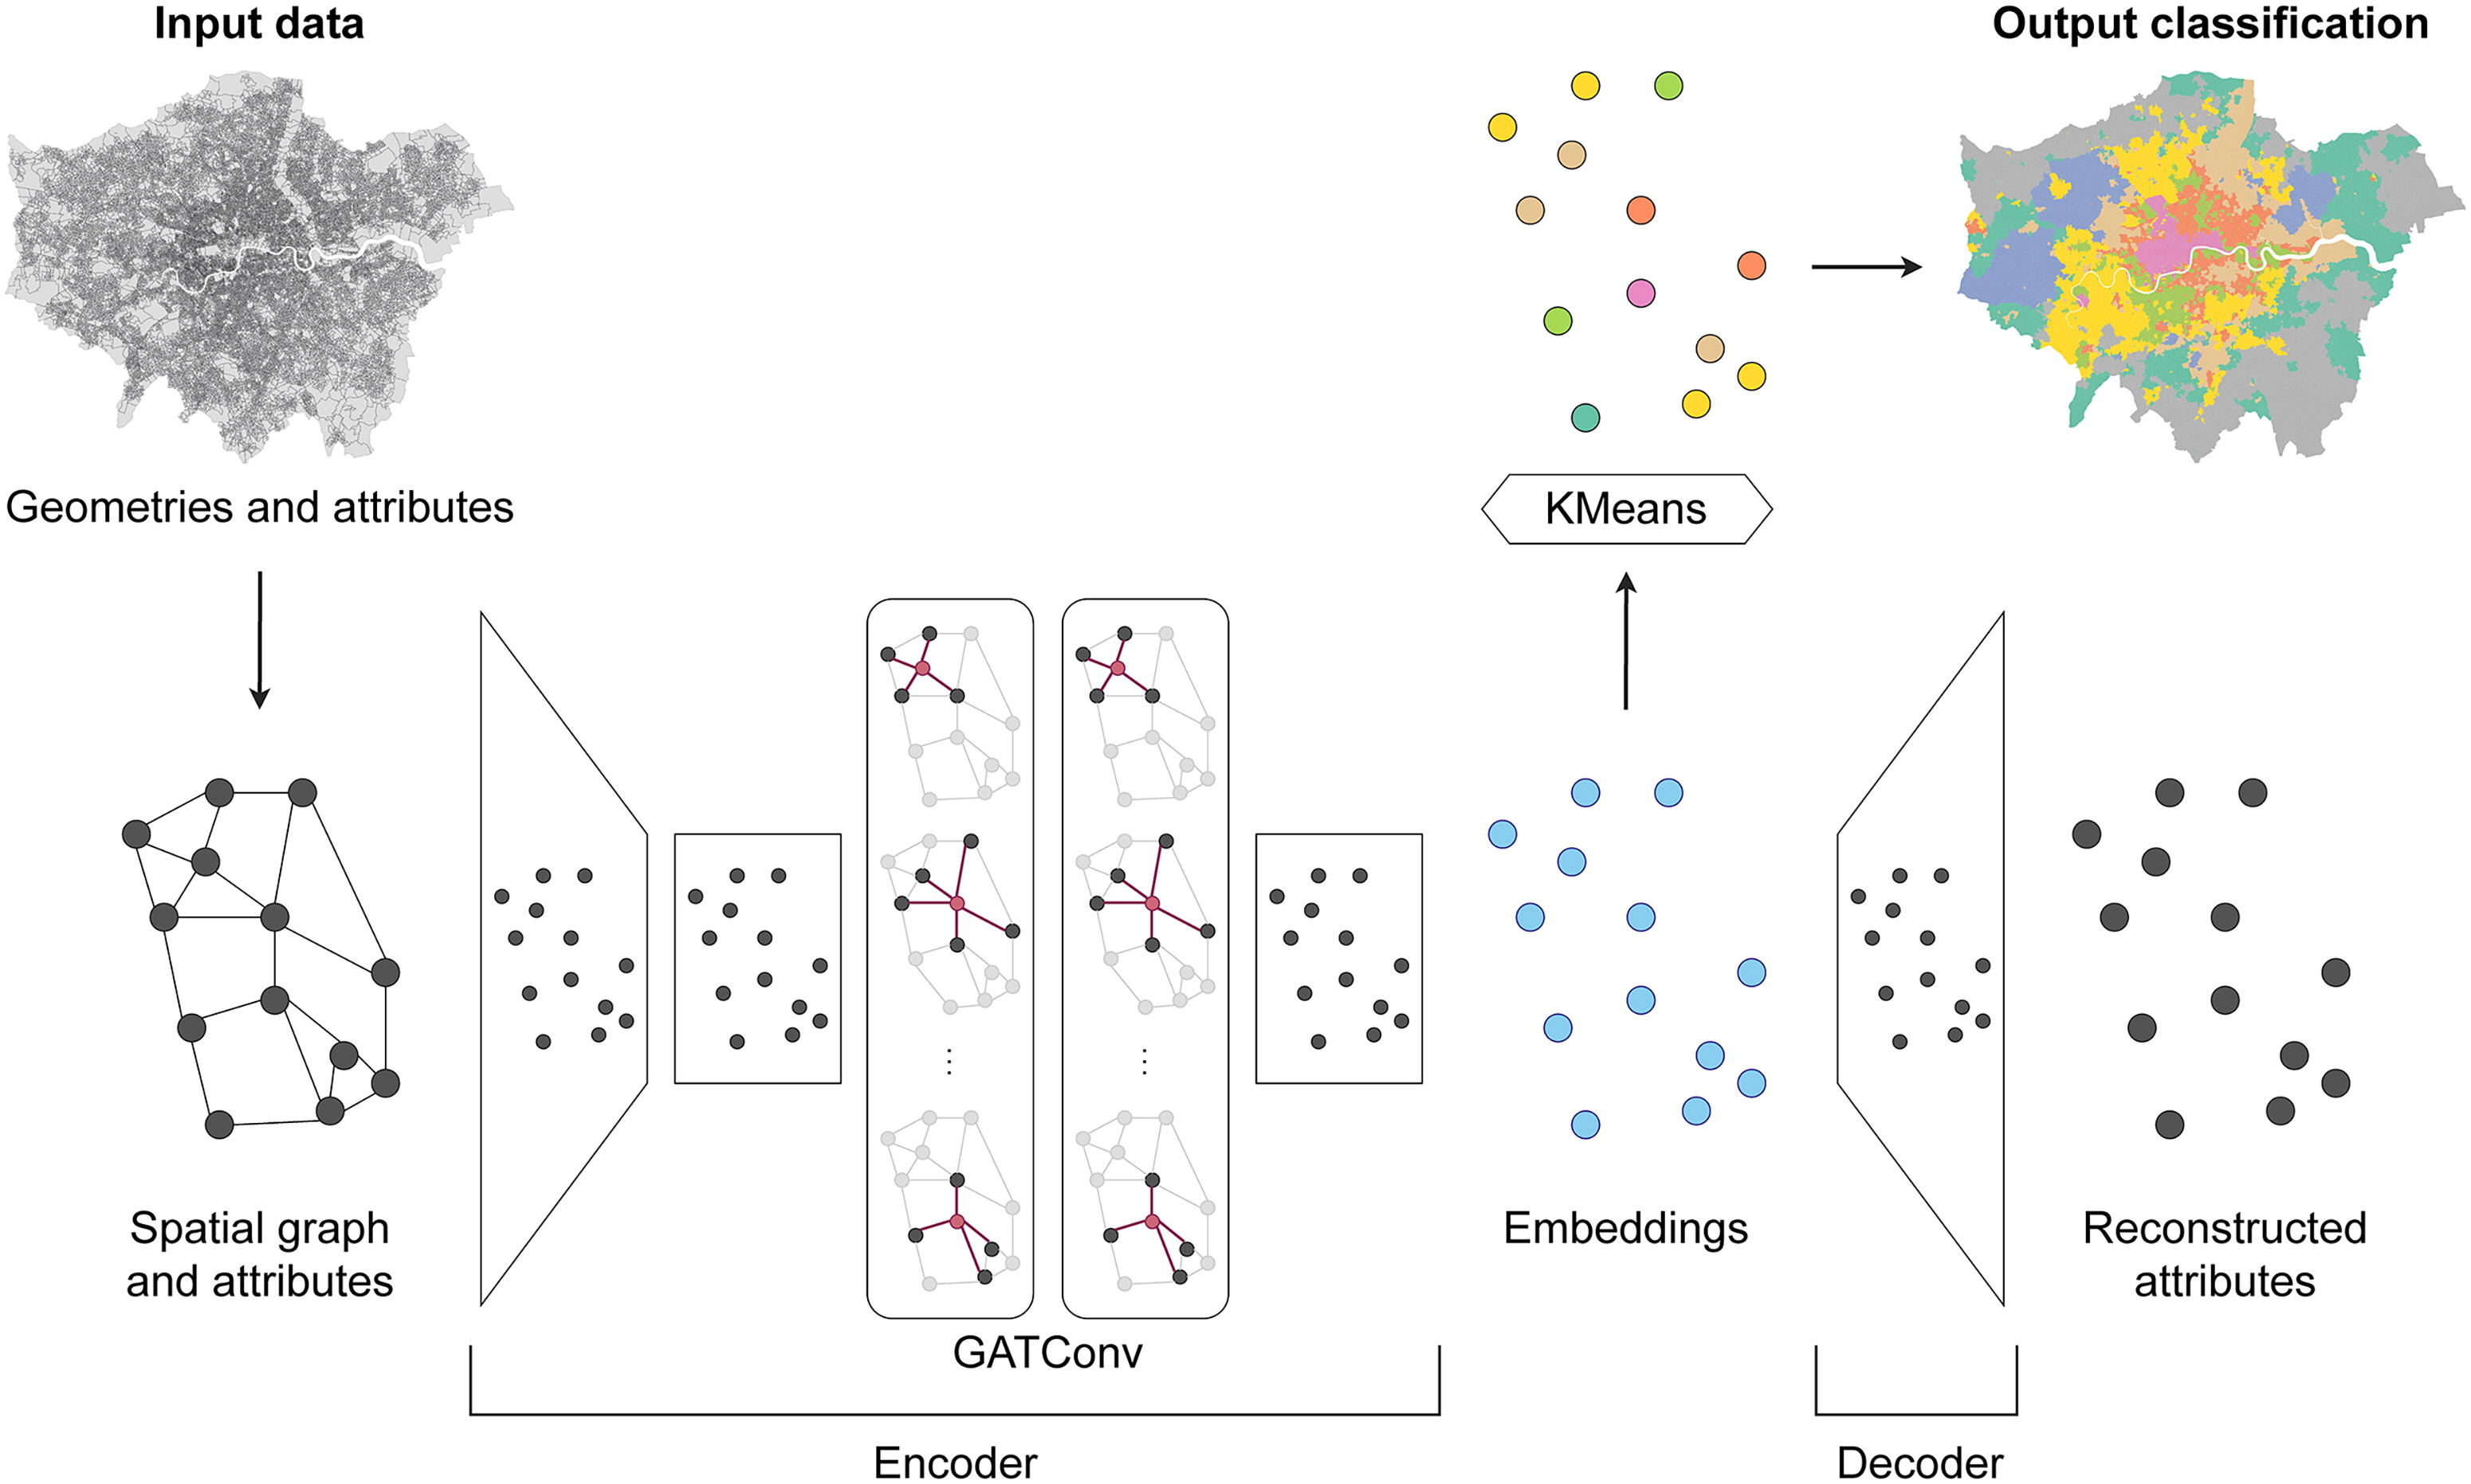
\includegraphics[width=0.4\textwidth]{../images/de_sabbata_and_liu_2023.jpg} % citation removed
        \end{center}       
    \end{itemize}
\end{frame}

\begin{frame}
    \frametitle{GNNs in Geographic Data Science (3/3)}
    \begin{itemize}
        \item \textbf{Example: Predicting Urban Functions by Forms} \parencite{chen_2025}
        \begin{itemize}            
            \item \textbf{Data:} Boston (nodes: 98,331 buildings, edges: Delaunay triangulation) 
            \item \textbf{Features:} Node: morphological metrics (size, shape, orientation, density), edge: distances
            \item \textbf{Task:} Predict urban functions using urban morphological graphs
            \item \textbf{Finding:} Proposed model effectively revealed high-order relationships between urban forms and functions
        \end{itemize}
        \begin{center}
            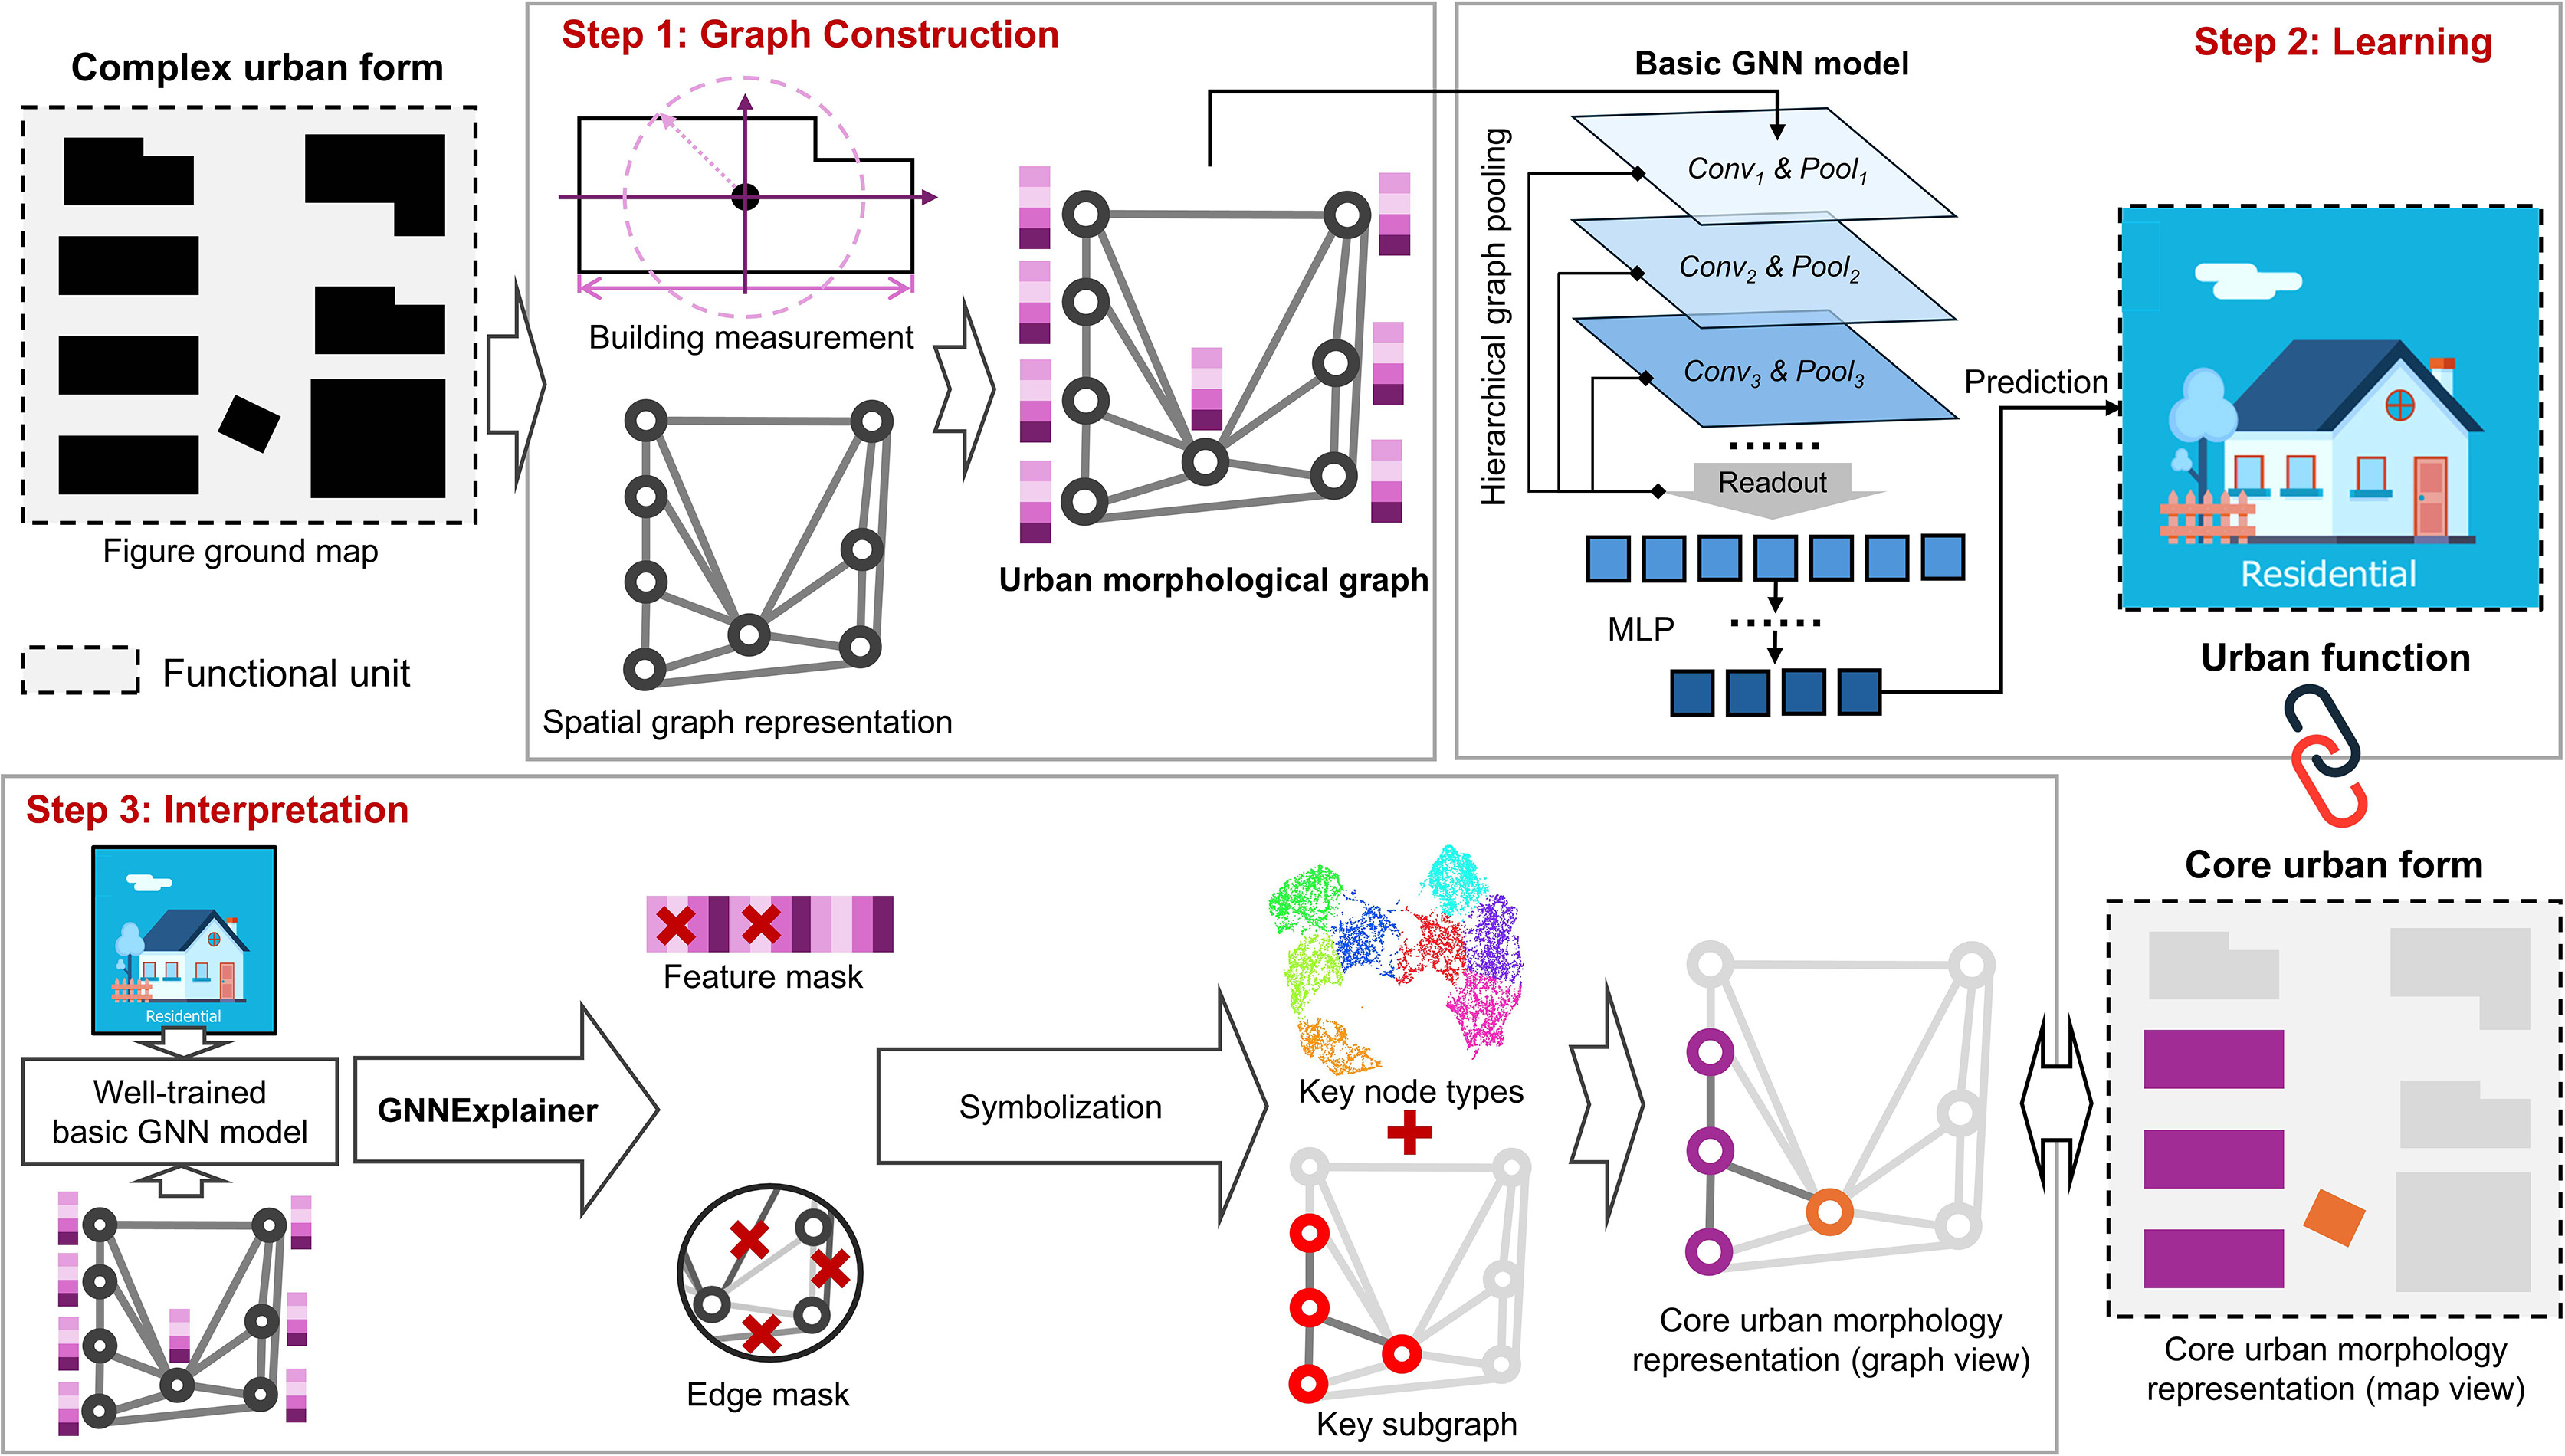
\includegraphics[width=0.5\textwidth]{../images/chen_et_al_2025.jpg}
        \end{center}
    \end{itemize}
\end{frame}

\section{Tech Demo} % Section title updated to match Agenda
\begin{frame}
    \frametitle{Tech Demo in Google Colab}
    \begin{itemize}
        \item Implementing GNNs with PyTorch Geometric (PyG):
        \begin{itemize}
            \item Popular library built on PyTorch.
            \item Efficient handling of sparse graph data.
            \item Provides standard GNN layers (GCN, GAT, etc.) and benchmark datasets.
        \end{itemize}
        \begin{center}
            
\includegraphics[width=0.3\textwidth]{../images/PyG.png} % Consider citing PyG paper/website
        \end{center}
        \item Demo Outline:
            \begin{itemize}
                \item Loading a sample graph dataset (e.g., Cora citation network or a simple geographic one).
                \item Defining a GCN model using PyG layers.
                \item Training the model for a node classification task.
                \item Visualizing node embeddings (optional).
            \end{itemize}
        \item Demo Link: \href{https://colab.research.google.com/drive/1f6l3cIVc29mkhdtNykn5lPy_W3_7RssL?usp=sharing}{Click here} % Clickable hyperlink
    \end{itemize}
\end{frame}

\begin{frame}[allowframebreaks]{References}
    \printbibliography
\end{frame}

\end{document}
